%! Author = niko
%! Date = 23/10/2023

% Preamble
\documentclass[../main]{subfiles}
\usepackage{glossaries}

% Document
\begin{document}

\newcommand{\tested}{\textsc{test}ed }
\newcommand{\Tested}{\textsc{Test}ed }

\chapter{\Tested{} deel 1, tijdelijke titel}
\label{ch:tested-deel-1-tijdelijke-titel}

This chapter describes the internal mechanisms and workings of \tested{}.
It begins with an overview of the ``architectural'' or conceptual design of \tested{}.
This is followed by a detailed look at the evaluation process: how a submission is evaluated using \tested{}.
Afterwards, we touch upon programming language support in \tested{}.

How a test suite is written is handled elsewhere.
TODO: link once written.

\section{Conceptual design}
\label{sec:conceptual design}

The main idea behind a programming-language-independent test framework is that an exercise designer can write a single test suite for a programming exercise, while the test framework is still able to evaluate submissions in multiple programming languages.

TESTed implements this concept using code generation.
This means that TESTed converts the test suite on the fly suite into the programming language of the submission.
It also takes care of the various aspects of the evaluation process: compiling the submitted code, executing the submission together with the test code, interpreting the results, and generating feedback.

While some parts of the evaluation process are obviously programming-language-specific, such as generating the test code, a lot of parts are not.
For example, creating an execution plan or interpreting the test results and generating the feedback are not specific to any one programming language.
Therefore, the language-specific aspects are isolated in language modules, as illustrated in~\cref{fig:conceptual-design}.

\begin{figure}[t]
    \centering
    \includestandalone{concept}
    \caption{
        Conceptual design of TESTed, with colors indicating different programming languages.
        The framework consists of a set of Python packages and modules.
        These can be categorized as the core package and a set of programming-language-specific modules.
        The input for TESTed consists of a test suite, together with a submitted solution in one of the supported languages
        The output is the generated feedback.
    }
    \label{fig:conceptual-design}
\end{figure}

\marginnote{
    A Python module is simply a \texttt{.py} file, while a Python package is a folder containing modules.
}
TESTed is written in Python and organized into a set of Python modules and packages.
An import package is the \emph{core} package, which contains modules that are responsible for all language-independent tasks, such as scheduling tests.
This is discussed in TODO.
In most cases, the core is also responsible for checking the collected test results and generating the feedback.
This is discussed in TODO.

All aspects that are specific to one programming language are bundled in one package.
These language-specific modules take care of all language-specific tasks, such as compiling submissions, executing submissions, and handling language-specific data types, expressions, and statements.
These modules are discussed in TODO.

Since the language-specific code is limited to these modules, this offers benefits for adding support for new programming languages to TESTed, see TODO.

TESTed requires a test suite for a programming exercise and a possible solution that needs to be evaluated as input.
The structure of the test suite is discussed in-depth in TODO.
As a result of its evaluation, TESTed outputs a feedback report as has been illustrated with some examples in the previous section. TODO


\section{Test suite structure}
\label{sec:test-suite-structure}

A test suite for TESTed is a hierarchical structure with three levels:

\marginnote{
    Since TESTed was originally developed for use with Dodona, these levels are equivalent to the Dodona levels tab, contexts and testcases (which contain tests).
}

\begin{enumerate}
    \item Units are the top-level grouping mechanism.
          It allows grouping of logically related testcases together.
    \item Testcases are the basic building blocks of a test suite.
          A testcase is a set of dependent tests.
          Testcases are independent of each other.
    \item Tests are the lowest level.
          A test consists of some input and a series of checks about different side effects or results (i.e.\ return values, standard out, standard error, exit codes or exceptions).
          Each output check is also called a script (since the input together with the output checks creates the script of a test).
\end{enumerate}

This structure mirrors the output generated by TESTed.
For example, the executed input for each test is also included in the output.
A possible visualization of these levels is given in~\cref{fig:dodona}, which shows the output rendered in Dodona.
TODO: reference

\begin{figure}
    \centering
    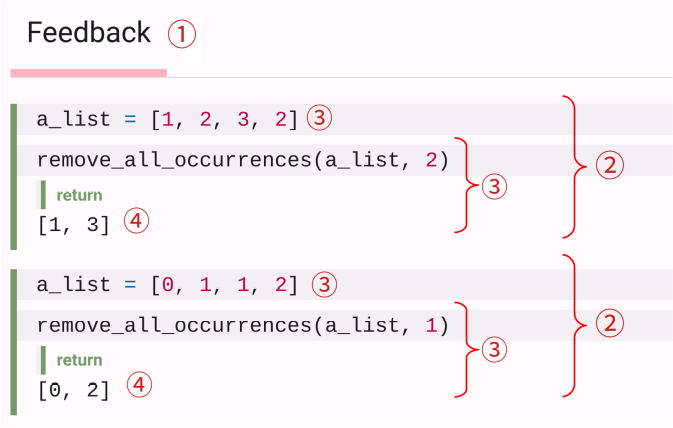
\includegraphics[scale=0.4]{dodona-rendering}
    \caption{A way to visually render the feedback (as done in Dodona resulting from evaluating a submission (in Python) with the test suite from TODO. There are four levels: \CircledText{1} units, \CircledText{2} testcases, \CircledText{3} tests and \CircledText{4} the scripts. Here, each testcase consists of two tests, the first of which has no script, while the second has one script (the expected return value).}
    \label{fig:dodona}
\end{figure}

TODO: add dataserialisation somewhere, perhaps own chapter

\section{Evaluating submissions}\label{sec:evaluating-submissions}

The input for the evaluation process is a test suite and a submission, which is typically provided by the judge platform in which TESTed runs (or can be provided manually if TESTed is run on the command line).
A general overview is given in~\cref{subsec:evaluation-process}.
Other subsections dive into more detail of individual parts of the process.

\subsection{Evaluation process}\label{subsec:evaluation-process}

We can now take a look at the complete evaluation process used by TESTed when evaluating a submission (a schematic is~\cref{fig:flow}).
The very first step in the evaluation process is checking if the exercise is solvable in the programming language of the submission (see~\cref{subsec:solvability-and-correctness-checks}).
Next, in the first step of the actual evaluation, the test suite is partitioned into compilation and execution units, as described in~\cref{subsec:execution-planning}.
For each of these units, the relevant code is generated and the resulting test code is compiled, as explained in~\cref{subsec:code-generation}.
The code is generated in the programming language of the submission.
This code generation is the bulk of language-specific code in TESTed, whose design and implementation are discussed in Programming-language-specific modules (TODO).

After compilation, each resulting executable contains one or more execution units.
These are then all executed, and the side effects (such as exceptions, stdout, stderr, etc.) and results (i.e.\ return values) are recorded.
These results are then checked for correctness against the test suite (see TODO).
This results in the feedback, which is returned by TESTed.

TESTed also has a step where static analysis is possible on the submission.
\marginnote{Examples include \texttt{ESLint}, \texttt{pylint} or \texttt{hlint}.}
Currently, all supported programming languages use this step to run a linter on the submission, the results of which are also included in the feedback as code annotations. SEE X.

\begin{figure}
    \centering
    \includestandalone{flow}
    \caption{
        The evaluation process of TESTed.
        The input consists of a submission and a test suite.
        After the planning phase, test code is generated, compiled, and executed.
        These results are then checked, which produces the final feedback.
        Separately, a linter runs on the submission, and its results are also included in the feedback.
    }
    \label{fig:flow}
\end{figure}

\subsection{Solvability and correctness checks}\label{subsec:solvability-and-correctness-checks}

The first step in the evaluation process is checking if the test suite is usable for the programming language of the submission.
This might not be the case for a number of reasons, the three main ones being:

\begin{itemize}
    \item The exercise designer has limited in which programming languages the exercise may be solved.
    \item The test suite uses constructs that are not supported by the programming language of the solution.
          For example, if the test suite uses object-oriented programming, the exercise will not be solvable in C or Haskell.
    \item The test suite contains programming-language-specific code but does not provide code for the programming language of the submission.
          For example, it is possible to manually provide the test code.
\end{itemize}

Additionally, there are some correctness checks, for example, on the syntax of the test suite.

\subsection{Execution planning}\label{subsec:execution-planning}

The next step is planning the execution of the evaluation.
As discussed before, a test suite contains a number of testcases, which must be independent of each other.
This allows TESTed to implement optimisations to improve performance.

TESTed partitions the test suite into compilation units (a set of testcases that are compiled together), which are in turn partitioned into execution units (a set of testcases that are executed together).
While different compilation units cannot be executed as one execution unit, it is possible that one compilation unit represents multiple execution units.

\begin{figure}
    \begin{subfigure}{\textwidth}
        \centering
        \includestandalone{planning-1}
        \caption{
            A schematic representation of the test suite.
            The test units are represented with green boxes, while the testcases (denoted as C\textsubscript{$n$}) are black boxes.
            In the subsequent figures, we leave the test suite box out to simplify the image.
        }
        \label{fig:planning-suite}
    \end{subfigure}
    \par\bigskip
    \begin{subfigure}{\textwidth}
        \centering
        \includestandalone{planning-2}
        \caption{
            The two possibilities for compilation units (denoted by red boxes).
            The upper scheme (with one compilation for the whole test suite) is always tried first.
            If this fails, each test unit becomes a compilation unit (the red boxes thus overlap with the green ones in the figure).
        }
        \label{fig:planning-compilation}
    \end{subfigure}
    \par\bigskip
    \begin{subfigure}{\textwidth}
        \centering
        \includestandalone{planning-3}
        \caption{
            Two possibilites execution unit partitionings (denoted by blue boxes), depending on the compilation units.
            In the first paritioning, there is a single compilation unit that is split into three execution units.
            The second partitioning cannot use the same execution units, as an execution unit cannot comprise multiple compilation units.
        }
        \label{fig:planning-execution}
    \end{subfigure}
    \caption{Schematic representation of the planning steps.}
\end{figure}

\subsubsection{Performance impact of the planning}

If performance was not relevant, the easiest execution plan would be to compile and execute each testcase individually.
After all, they are independent of each other, and separate compilation and execution would ensure that independence.

However, this would be prohibitively slow: a test suite with fifty test cases would need fifty compilation steps and fifty execution steps.
Creating an execution plan is thus intended to improve performance, which is done in two ways:

\marginnote{The final execution units are also executed in parallel, which is described in TODO.}
\begin{enumerate}
    \item Reducing the number of compilation units.
    \item Reducing the number of execution units.
\end{enumerate}

\subsubsection{Compilation units}

First, TESTed tries to use a single compilation unit for the whole test suite.
This is achieved by creating a program that accepts an argument to indicate the execution that should be run.

In programming languages without an explicit compilation step, the compilation is no more than a syntax check.
\marginnote{
    For example, our JavaScript implementation uses \texttt{node -c}.
}
In compiled languages, the compilation is often much stricter, for example, failing if a non-existing function is used.

Techniques used to improve performance must be weighed against the usability.
For example, consider an exercise where students must implement two or three functions.
Students might often implement the first function and submit their solution.
With a single compilation unit, a compilation would occur, since our test code calls functions that do not exit.
This will prevent the first function from being evaluated, even if it was correct.

To prevent this, if the compilation of the whole test suite fails, TESTed falls back to using one compilation unit per unit in the test suite.
These two approaches are illustrated in~\cref{fig:planning-compilation}.

This is why a unit is intended to be a set of logically related testcases.
Continuing with the example from before, there might be a separate unit for each function the exercise requires.
Going more fine-grained, that is compiling each testcase individually, does not seem useful.
While potentially providing faster feedback, the performance impact is not worth it.

Compiling at the unit level is a good compromise between fain-grained compilation (thus allowing more of the submission to be evaluated) and performance (the more compilation units, the slower the evaluation will be).

\subsubsection{Execution units}

Next, the compilation units from the previous steps are partitioned into execution units.
\marginnote{
All programming languages, including the non-compiled ones, are handled the same way.
This allows the most consistency between programming languages.
}
Each execution unit can be at most one compilation unit: we cannot execute multiple compilation units together,
as each compilation unit results in a separate executable.
However, depending on the testcases inside a compilation unit, we can (and do) execute a compilation unit multiple times.

For performance reasons, the ideal partitioning would be a single execution unit for the whole test suite.
However, this prevents certain types of exercises from being evaluated correctly.
Therefore, a new execution unit is started based on the type of testcase: if a testcase has stdin, command line arguments, or an explicit check for the exit code, a new execution unit is started.

\subsection{Generating code}\label{subsec:code-generation}

Depending on the execution plan, the appropriate code is generated for the test suite.
In concept, this step converts the programming-language-independent test suite into actual source code, in the programming language of the test suite.
For example, for a submission in JavaScript, the generated code will also be in JavaScript.

As shown in~\cref{fig:flow}, code is generated for each compilation unit.
The main purpose of the generated code is to execute the tests specified in the test suite.
For this reason, we also call the generated code the \emph{test code}.

Besides executing the tests from the test suite, the generated code also contains some \emph{ceremonial} code required by TESTed.
Some examples of this code are:

\begin{itemize}
    \item As mentioned in~\cref{subsec:execution-planning}, in the ideal case, we only have one compilation unit and thus one executable for the whole test suite.
     We thus generate a wrapper that executes the correct execution unit based on some parameter (e.g.\ \texttt{./testcode "unit1"}).
    \item The generated code includes serialization capabilities (see TODO), to convert captured values into the internal data format used by TESTed.
    \item The tests are wrapped in code that captures side effects and values, such as exceptions, return values, etc.
\end{itemize}

This code generation is the main task of the programming-language-specific modules, discussed in TODO.

\subsection{Executing test code}\label{subsec:executing-test-code}

After the test code has been generated and compiled into executables, these executables are then (logically) executed.

During this execution, special care is taken to ensure that the executions are independent of each other.
As discussed in TODO, execution happens in a special directory called the \emph{workdir} (from working directory).
For each execution, TESTed creates a new subdirectory and copies the relevant files into that subdirectory.
The execution then happens in the subdirectory.

The independence of execution is useful to prevent other executions from interfering.
For example, consider an erroneous submission for an exercise where data is provided in a file.
If the submission overwrites or changes the file by accident, subsequent executions would use the modified file.
However, since the file is copied into each subdirectory, this scenario is prevented.

A second benefit of the independent executions is the ability to execute in parallel.
This option is disabled by default, due to the way Dodona works (TODO link).
However, even in that scenario, this improves the performance of certain exercises, for example those exercises that use scripts, command lines, or main functions.

The astute reader might wonder how this is implemented, since TESTed is written in Python, a language whose default implementation (CPython) has an infamous global interpreter lock (or GIL).
This means that at any one time, only one thread can execute Python code.
\marginnote{
Work is ongoing to improve the situation, or even remove the GIL, as PEP 703: \url{https://peps.python.org/pep-0703/}
}
One workaround is to use multiple processes: this sidesteps the issue entirely, but using multiple processes is fairly heavy in general.
This is even truer in TESTed, as executing the test code already happens in a separate process.

This leads directly to the solution in TESTed: since the test code is executed in a separate process, the GIL does not apply.
Most of the time is spent waiting on results from a subproces.

\subsection{Checking the test results}\label{subsec:checking-results}

The code responsible for checking wheter test results (return values, stdout, etc.) are correct is called an oracle. TODO referentie.
TESTed supports three types of oracles, which can be divided into two categories.
The first two oracle types are generic, meaning that they are programming language independent.
These are also explained in TODO, where the focus lies on using the oracles.
The third oracle type is a programming-language-dependent oracle.

The two generic oracles are the built-in oracles and the programmed oracles.
The first are oracles which are, as the name implies, built into TESTed.
These are rather simple, but should suffice for most exercises.
Currently, the following oracles are included:

\begin{itemize}
    \item The text oracle.
          This oracle compares two strings and is used for stdout and stderr.
          The oracle has some options, for example, to ignore trailing whitespace, to attempt to parse the text as floating point numbers or case sensitivity.
          The expected value can be provided either as a string, or as a file, in which case the contents of said file are used as the string.
    \item The file oracle.
          This allows comparison between two files, either comparing the whole file, or comparing the file line-by-line.
          When comparing line-by-line, the text oracle is used, so the same options can be provided.
    \item The return value oracle.
          This oracle compares two values (see TODO for the test values).
          The oracle does more than just a value comparison: the types of the data are also compared, using the TESTed type system (see TODO for how this works).
    \item The exception oracle.
          This allows checking exceptions.
          By default, only the message of the exception is checked, as the type of an exception is programming language dependent.
          However, the oracle does have an option to provide the expected type for the different programming languages, in which case those will be checked as well.
          Do note that checking the type happens with a string-based check, meaning that if a student implements a custom exception with the same name, it will pass the check.
\end{itemize}

There are a number of scenarios where the built-in oracles are not enough to properly check an exercise.
One such example is an exercise where dynamic data is used, for example a return value that depends on the current date.
Another example is a random or otherwise nondeterministic return value, where the value must satisfy some conditions.
Finally, sometimes the exercise is static, but you want to provide some exercise-specific feedback.
For example, if the exercise is to generate an SVG, you might want to show that SVG to students.

For these scenarios, a programmed oracle can be used.
Such an oracle is, in essence, an extension of the built-in oracles: instead of using a built-in oracle, TESTed will call the exercise-provided oracle.
See TODO for how to use such an oracle.
TODO: zeggen dat ze enkel in Python bestaan?

We have not yet encountered an exercise not covered by the generic oracles; however, it is not hard to imagine exercises that cannot be checked using those.
As such, TESTed provides an escape hatch: a programming-language-specific oracle.
These oracles are run together with the generated test code and skip the serialization pipeline.
They are therefore not subject to the serialization limits of TESTed.
An example could be an exercise where a function returns an instance of a custom class.

The big downside to using these oracles is that they are programming-language-specific.
The oracle thus has to be implemented in each programming language the exercise supports.
These oracles are therefore only provided as an escape route for language-specific expressions, statements, and data types.

\subsection{Static analysis of the submission}\label{subsec:static-analysis-of-the-submission}

TESTed also provides a way to perform exercise-independent static analysis on the submission as part of the evaluation process.
TODO: references naar linters en dat ze goed werken.
Currently, all supported languages (except C\#, where the compiler acts a linter) use an external linter to generate additional feedback, see~\cref{tab:linters}.
While this feedback is generally not specific to an exercise, nor is its main goal to check the correctness of the submission, it does provide additional hints to students on how to improve their submission.

TODO: refereren waar mogelijk
\begin{table}[h]
    \centering
    \caption{Overview of the used linters in TESTed.}
    \label{tab:linters}
    \begin{tabular}{|l|l|}
        \hline
        Programming language & Linter \\
        \hline
        Bash & Shellcheck  \\
        C & Cppcheck \\
        Haskell & HLint \\
        Java & Checkstyle \\
        JavaScript & ESLint \\
        Kotlin & Ktlint \\
        Python & Pylint \\
        \hline
    \end{tabular}
\end{table}

\subsection{Feedback}\label{subsec:feedback}

The last step of the evaluation process is to return the generated feedback.
The feedback has the same structure as the test suite (\cref{sec:test-suite-structure}).
The format is the partial feedback format from Dodona TODO ref.
However, there are almost no Dodona-specific features in this format.

The format is named \emph{partial} since it is streaming JSON format.
This means that the output is a stream of JSON objects, instead of one big JSON object.

\marginnote{There also exists RFC 7464~\cite{rfc7464}, where each JSON object is started by a \emph{record seperator} character and ended with a newline. This is a relatively new format that doesn't seem to be widely-used.}
TODO: cite this?.
TESTed uses newline-delimited JSON\@.
Two equivalent \emph{specifications} exist for this format: NDJSON (Newline-Delimited JSON\footnote{\url{https://ndjson.org/}}) and JSON Lines\footnote{https://jsonlines.org/}.
The format itself is simple: JSON objects are separated by a newline, and each line is a valid JSON object.

The structure of the feedback is indicated by commands, with \emph{start} commands to begin a new level in the hierarchy and \emph{close} commands to finish a level.
\cref{lst:tested-output-example} contains the output from TESTed that resulted in the feedback as shown in~\cref{fig:dodona}.

\begin{listing}
    \begin{minted}{json}
        {"command": "start-judgement"}
        {"command": "start-tab", "title": "Feedback"}
        {"command": "start-context"}
        {"command": "start-testcase", "description": "a_list = [1, 2, 3, 2]"}
        {"command": "close-testcase"}
        {"command": "start-testcase", "remove_all_occurrences(a_list, 2)"}
        {"command": "start-test", "expected": "[1, 3]", "channel": "return"}
        {"command": "close-test", "generated": "[1, 3]", "status": "correct"}
        {"command": "close-testcase"}
        {"command": "close-context"}
        {"command": "start-context"}
        {"command": "start-testcase", "description": "a_list = [0, 1, 1, 2]"}
        {"command": "close-testcase"}
        {"command": "start-testcase", "remove_all_occurrences(a_list, 1)"}
        {"command": "start-test", "expected": "[0, 2]", "channel": "return"}
        {"command": "close-test", "generated": "[0, 2]", "status": "correct"}
        {"command": "close-testcase"}
        {"command": "close-context"}
        {"command": "close-tab"}
        {"command": "close-judgement"}
    \end{minted}
    \caption{
        Example of the output generated by TESTed, which is rendered in~\cref{fig:dodona}.
        Note that the names of the levels are the Dodona levels (tab, contex and testcase), instead of unit, testcase and script.
        As before, each testcase consists of two tests, the first of which has no script, while
        the second has one script (the expected return value).
    }
    \label{lst:tested-output-example}
\end{listing}





\end{document}
